\documentclass[11pt,a4paper]{report}
\usepackage[textwidth=37em,vmargin=30mm]{geometry}
\usepackage{calc,xunicode,amsmath,amssymb,paralist,enumitem,tabu,booktabs,datetime2,xeCJK,xeCJKfntef,listings}
\usepackage{tocloft,fancyhdr,tcolorbox,xcolor,graphicx,eso-pic,xltxtra,xelatexemoji}

\newcommand{\envyear}[0]{2025}
\newcommand{\envdatestr}[0]{2025-08-30}
\newcommand{\envfinaldir}[0]{webdb/2025/20250830/final}

\usepackage[hidelinks]{hyperref}
\hypersetup{
    colorlinks=false,
    pdfpagemode=FullScreen,
    pdftitle={Web Digest - \envdatestr}
}

\setlength{\cftbeforechapskip}{10pt}
\renewcommand{\cftchapfont}{\rmfamily\bfseries\large\raggedright}
\setlength{\cftbeforesecskip}{2pt}
\renewcommand{\cftsecfont}{\sffamily\small\raggedright}

\setdefaultleftmargin{2em}{2em}{1em}{1em}{1em}{1em}

\usepackage{xeCJK,xeCJKfntef}
\xeCJKsetup{PunctStyle=plain,RubberPunctSkip=false,CJKglue=\strut\hskip 0pt plus 0.1em minus 0.05em,CJKecglue=\strut\hskip 0.22em plus 0.2em}
\XeTeXlinebreaklocale "zh"
\XeTeXlinebreakskip = 0pt


\setmainfont{Brygada 1918}
\setromanfont{Brygada 1918}
\setsansfont{IBM Plex Sans}
\setmonofont{JetBrains Mono NL}
\setCJKmainfont{Noto Serif CJK SC}
\setCJKromanfont{Noto Serif CJK SC}
\setCJKsansfont{Noto Sans CJK SC}
\setCJKmonofont{Noto Sans CJK SC}

\setlength{\parindent}{0pt}
\setlength{\parskip}{8pt}
\linespread{1.15}

\lstset{
	basicstyle=\ttfamily\footnotesize,
	numbersep=5pt,
	backgroundcolor=\color{black!5},
	showspaces=false,
	showstringspaces=false,
	showtabs=false,
	tabsize=2,
	captionpos=b,
	breaklines=true,
	breakatwhitespace=true,
	breakautoindent=true,
	linewidth=\textwidth
}






\newcommand{\coverpic}[2]{
    % argv: itemurl, authorname
    Cover photo by #2~~(\href{#1}{#1})
}
\newcommand{\makeheader}[0]{
    \begin{titlepage}
        % \newgeometry{hmargin=15mm,tmargin=21mm,bmargin=12mm}
        \begin{center}
            
            \rmfamily\scshape
            \fontspec{BaskervilleF}
            \fontspec{Old Standard}
            \fontsize{59pt}{70pt}\selectfont
            WEB\hfill DIGEST
            
            \vfill
            % \vskip 30pt
            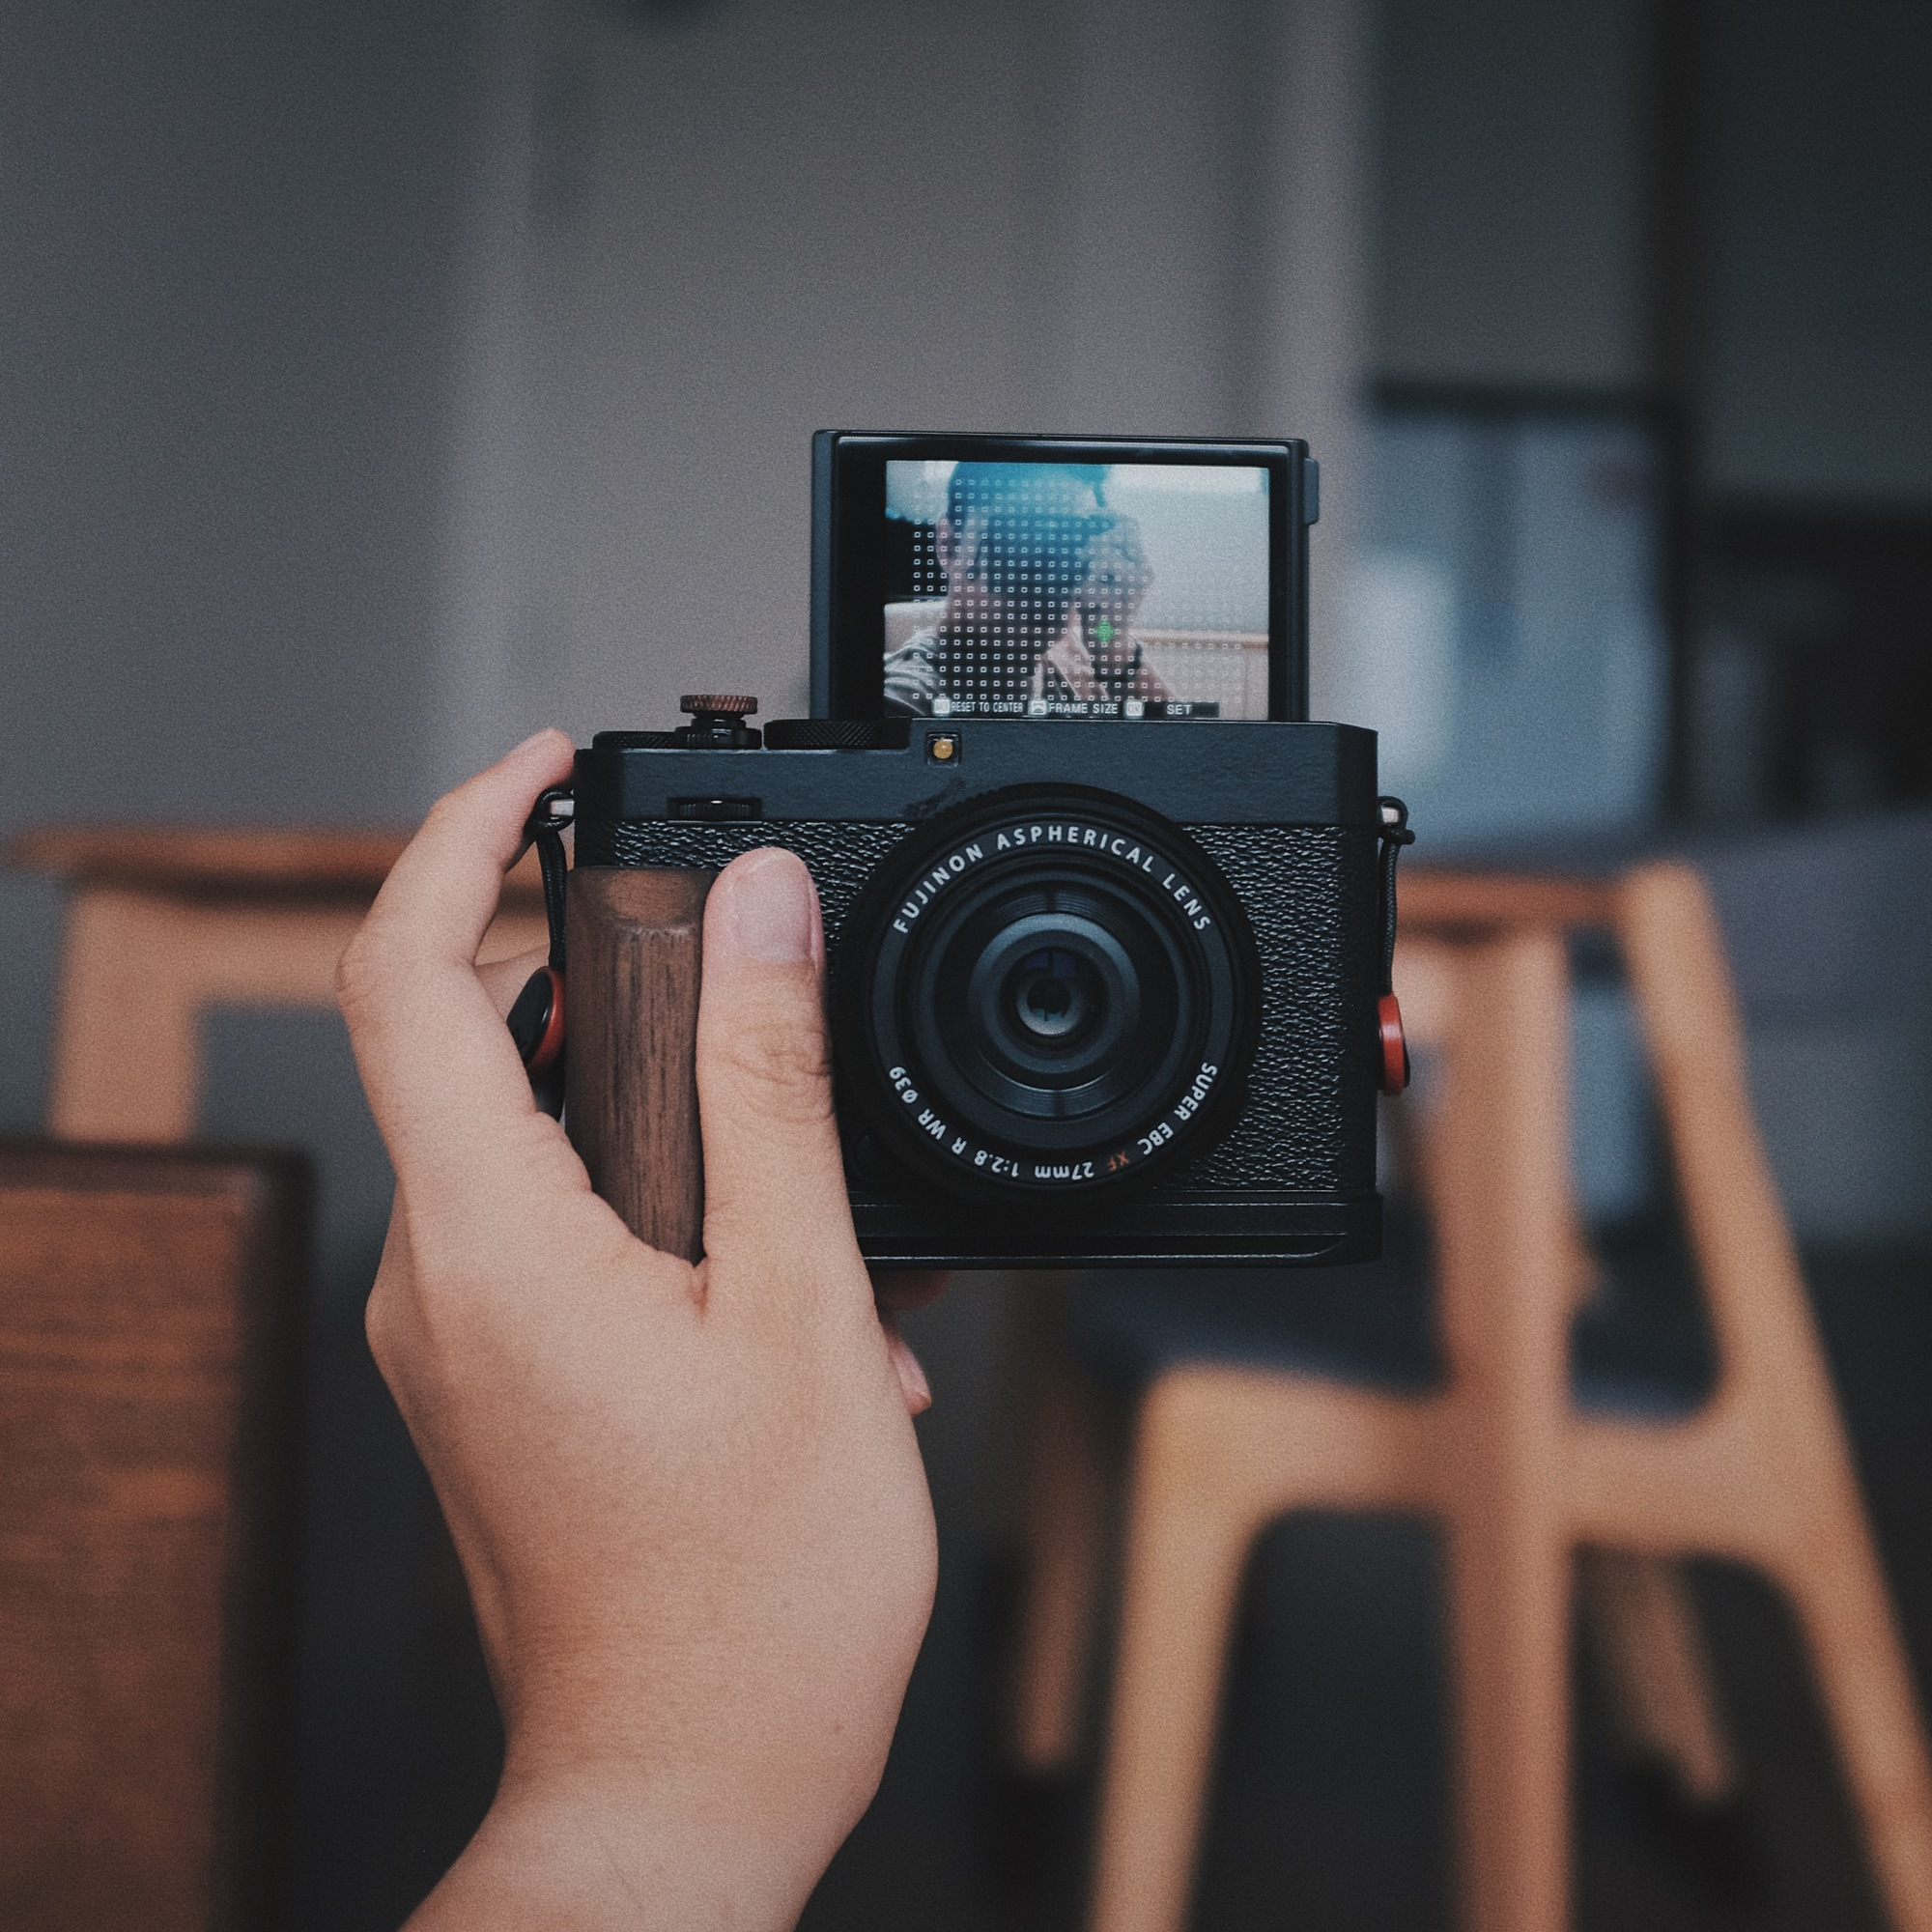
\includegraphics[width=\linewidth]{\envfinaldir/coverpic-prod.jpg}\par
            % \vskip 30pt
            \vfill

            \normalsize\rmfamily\scshape
            \copyright{} The Web Digest Project \hfill\large \envdatestr
        \end{center}
    \end{titlepage}
    % \restoregeometry
}
\newcommand{\simplehref}[1]{%
    \textcolor{blue!80!green}{\href{#1}{#1}}%
}
\renewcommand{\contentsname}{\center\Huge\sffamily\bfseries Contents\par\vskip 20pt}
\newcounter{ipartcounter}
\setcounter{ipartcounter}{0}
\newcommand{\ipart}[1]{
    % \vskip 20pt
    \clearpage
    \stepcounter{ipartcounter}
    \phantomsection
    \addcontentsline{toc}{chapter}{#1}
    % \begin{center}
    %     \Huge
    %     \sffamily\bfseries
    %     #1
    % \end{center}
    % \vskip 20pt plus 7pt
}
\newcounter{ichaptercounter}
\setcounter{ichaptercounter}{0}
\newcommand{\ichapter}[1]{
    % \vskip 20pt
    \clearpage
    \stepcounter{ichaptercounter}
    \phantomsection
    \addcontentsline{toc}{section}{\numberline{\arabic{ichaptercounter}}#1}
    \begin{center}
        \Huge
        \sffamily\bfseries
        #1
    \end{center}
    \vskip 20pt plus 7pt
}
\newcommand{\entrytitlefont}[1]{\subsection*{\raggedright\Large\sffamily\bfseries#1}}
\newcommand{\entryitemGeneric}[2]{
    % argv: title, url
    \parbox{\linewidth}{
        \entrytitlefont{#1}\par\vskip 5pt
        \footnotesize\ttfamily\mdseries
        \simplehref{#2}
    }\vskip 11pt plus 11pt minus 1pt
}
\newcommand{\entryitemGithub}[3]{
    % argv: title, url, desc
    \parbox{\linewidth}{
        \entrytitlefont{#1}\par\vskip 5pt
        \footnotesize\ttfamily\mdseries
        \simplehref{#2}\par\vskip 5pt
        \small\rmfamily\mdseries#3
    }\vskip 11pt plus 11pt minus 1pt
}
\newcommand{\entryitemAp}[3]{
    % argv: title, url, desc
    \parbox{\linewidth}{
        \entrytitlefont{#1}\par\vskip 5pt
        \footnotesize\ttfamily\mdseries
        \simplehref{#2}\par\vskip 5pt
        \small\rmfamily\mdseries#3
    }\vskip 11pt plus 11pt minus 1pt
}
\newcommand{\entryitemHackernews}[3]{
    % argv: title, hnurl, rawurl
    % \parbox{\linewidth}{
    %     \entrytitlefont{#1}\par\vskip 5pt
    %     \footnotesize\ttfamily\mdseries
    %     \simplehref{#3}\par
    %     \textcolor{black!50}{\href{#2}{#2}}
    % }\vskip 11pt plus 11pt minus 1pt
    \begin{minipage}{\linewidth}
            \entrytitlefont{#1}\par\vskip 5pt
            \footnotesize\ttfamily\mdseries
            \simplehref{#3}\par
            \textcolor{black!50}{\href{#2}{#2}}
    \end{minipage}\par\vskip 11pt plus 11pt minus 1pt
}







\begin{document}

\makeheader

\tableofcontents\clearpage




\ipart{Developers}
\ichapter{Hacker News}
\entryitemTwoLinks{Do the simplest thing that could possibly work}{https://news.ycombinator.com/item?id=45068091}{https://www.seangoedecke.com/the-simplest-thing-that-could-possibly-work/}

\entryitemTwoLinks{SQLite's documentation about its durability properties is unclear}{https://news.ycombinator.com/item?id=45066999}{https://www.agwa.name/blog/post/sqlite\_durability}

\entryitemTwoLinks{John Carmack's arguments against building a custom XR OS at Meta}{https://news.ycombinator.com/item?id=45066395}{https://twitter.com/ID\_AA\_Carmack/status/1961172409920491849}

\entryitemTwoLinks{The web does not need gatekeepers: Cloudflare's new ``signed agents'' pitch}{https://news.ycombinator.com/item?id=45066258}{https://positiveblue.substack.com/p/the-web-does-not-need-gatekeepers}

\entryitemTwoLinks{Wikipedia as a Graph}{https://news.ycombinator.com/item?id=45066060}{https://wikigrapher.com/paths}

\entryitemTwoLinks{Essential Coding Theory [pdf]}{https://news.ycombinator.com/item?id=45065705}{https://cse.buffalo.edu/faculty/atri/courses/coding-theory/book/web-coding-book.pdf}

\entryitemTwoLinks{Taco Bell rethinks AI drive-through after man orders 18,000 waters}{https://news.ycombinator.com/item?id=45065391}{https://www.bbc.com/news/articles/ckgyk2p55g8o}

\entryitemTwoLinks{Why AI Isn't Ready to Be a Real Coder}{https://news.ycombinator.com/item?id=45065343}{https://spectrum.ieee.org/ai-for-coding}

\entryitemTwoLinks{Deploying DeepSeek on 96 H100 GPUs}{https://news.ycombinator.com/item?id=45064329}{https://lmsys.org/blog/2025-05-05-large-scale-ep/}

\entryitemTwoLinks{Flunking my Anthropic interview again}{https://news.ycombinator.com/item?id=45064284}{https://taylor.town/flunking-anthropic}

\entryitemTwoLinks{Private equity snaps up disability services, challenging regulators}{https://news.ycombinator.com/item?id=45063972}{https://www.governing.com/management-and-administration/private-equity-snaps-up-disability-services-challenging-regulators}

\entryitemTwoLinks{Grok Code Fast 1}{https://news.ycombinator.com/item?id=45063559}{https://x.ai/news/grok-code-fast-1}

\entryitemTwoLinks{Sig Sauer citing national security to keep documents from public}{https://news.ycombinator.com/item?id=45063431}{https://practicalshootinginsights.com/eighth-circuit-fmeca-update/}

\entryitemTwoLinks{Some users have noticed settings that let Meta analyze and retain phone photos}{https://news.ycombinator.com/item?id=45062910}{https://www.zdnet.com/article/meta-might-be-secretly-scanning-your-phones-camera-roll-how-to-check-and-turn-it-off/}

\entryitemTwoLinks{If you have a Claude account, they're going to train on your data moving forward}{https://news.ycombinator.com/item?id=45062738}{https://old.reddit.com/r/LocalLLaMA/comments/1n2ubjx/if\_you\_have\_a\_claude\_personal\_account\_they\_are/}

\entryitemTwoLinks{Updates to Consumer Terms and Privacy Policy}{https://news.ycombinator.com/item?id=45062683}{https://www.anthropic.com/news/updates-to-our-consumer-terms}

\entryitemTwoLinks{Tesla said it didn't have key data in a fatal crash, then a hacker found it}{https://news.ycombinator.com/item?id=45062614}{https://www.washingtonpost.com/technology/2025/08/29/tesla-autopilot-crashes-evidence-testimony-wrongful-death/}

\entryitemTwoLinks{The Synology End Game}{https://news.ycombinator.com/item?id=45060920}{https://lowendbox.com/blog/they-used-to-be-good-but-now-theyve-turned-to-evil-the-synology-end-game/}

\entryitemTwoLinks{Strange CW Keys}{https://news.ycombinator.com/item?id=45060161}{https://sites.google.com/site/oh6dccw/strangecwkeys}

\entryitemTwoLinks{PSA: Libxslt is unmaintained and has 5 unpatched security bugs}{https://news.ycombinator.com/item?id=45060004}{https://vuxml.freebsd.org/freebsd/b0a3466f-5efc-11f0-ae84-99047d0a6bcc.html}


\ipart{Developers~~~~(zh-Hans)}
\ichapter{Solidot}
\entryitemGeneric{\hskip 0pt{}黄石公园内自由迁徙的野牛加强了草原的恢复力}{https://www.solidot.org/story?sid=82174}

\entryitemGeneric{\hskip 0pt{}美商务部长称将在区块链上发布经济数据}{https://www.solidot.org/story?sid=82173}

\entryitemGeneric{\hskip 0pt{}日本小镇考虑倡导每天仅使用智能手机两小时}{https://www.solidot.org/story?sid=82172}

\entryitemGeneric{\hskip 0pt{}FFmpeg 8 支持实时生成字幕}{https://www.solidot.org/story?sid=82171}

\entryitemGeneric{\hskip 0pt{}研究显示 AI 的普及与美国初级工作的减少相关}{https://www.solidot.org/story?sid=82170}

\entryitemGeneric{\hskip 0pt{}美国共和党人调查维基百科的自由主义偏见}{https://www.solidot.org/story?sid=82169}

\entryitemGeneric{\hskip 0pt{}用流行病学分析法国大革命}{https://www.solidot.org/story?sid=82168}

\entryitemGeneric{\hskip 0pt{}开源项目通常由一个人维护}{https://www.solidot.org/story?sid=82167}

\entryitemGeneric{\hskip 0pt{}Nothing 成为最新一家被发现用图库照片演示手机摄影能力的厂商}{https://www.solidot.org/story?sid=82166}

\entryitemGeneric{\hskip 0pt{}源自 ChatGPT 的常用词在人们的日常对话中也日益流行}{https://www.solidot.org/story?sid=82165}

\entryitemGeneric{\hskip 0pt{}三名台积电工程师因窃取 2 纳米工艺机密被起诉}{https://www.solidot.org/story?sid=82164}

\entryitemGeneric{\hskip 0pt{}印度屏蔽 Sci-Hub}{https://www.solidot.org/story?sid=82163}

\entryitemGeneric{\hskip 0pt{}《K-POP:猎魔女团》成为 Netflix 史上观看次数最多的电影}{https://www.solidot.org/story?sid=82162}

\entryitemGeneric{\hskip 0pt{}Windows 版本的 Word v2509 默认将文档保存到云端}{https://www.solidot.org/story?sid=82161}

\entryitemGeneric{\hskip 0pt{}GMP 项目报告 AMD CPU 烧毁事故}{https://www.solidot.org/story?sid=82160}

\entryitemGeneric{\hskip 0pt{} 开发者创新盛典 | NVIDIA 2025 Hackathon 年度总决赛报名即日启动!}{https://www.solidot.org/story?sid=82159}

\entryitemGeneric{\hskip 0pt{}韩国禁止中小学生课堂使用手机}{https://www.solidot.org/story?sid=82156}

\entryitemGeneric{\hskip 0pt{}Bluesky 成为科学社区的首选平台}{https://www.solidot.org/story?sid=82155}

\entryitemGeneric{\hskip 0pt{}AMD 称部分 X3D 烧毁是主板导致的}{https://www.solidot.org/story?sid=82153}

\entryitemGeneric{\hskip 0pt{}森林砍伐过去 20 年导致 50 万人死亡}{https://www.solidot.org/story?sid=82152}\ichapter{V2EX}
\entryitemGeneric{\hskip 0pt{}[推广] 活钱 29 | 信用卡提额:银行认可的七大技巧}{https://www.v2ex.com/t/1155900}

\entryitemGeneric{\hskip 0pt{}[生活] 七夕苦恼的兄弟们我去敌人内部开团了}{https://www.v2ex.com/t/1155899}

\entryitemGeneric{\hskip 0pt{}[酷工作] 现在做招聘的人这么卷}{https://www.v2ex.com/t/1155896}

\entryitemGeneric{\hskip 0pt{}[程序员] 一个 npm update 操作把服务搞崩了}{https://www.v2ex.com/t/1155895}

\entryitemGeneric{\hskip 0pt{}[路由器] 回归本质:大家给推荐一款路由器价格在 1000 上下}{https://www.v2ex.com/t/1155894}

\entryitemGeneric{\hskip 0pt{}[宽带症候群] 关于 PCDN 用户对 PT 用户的吸血}{https://www.v2ex.com/t/1155893}

\entryitemGeneric{\hskip 0pt{}[OpenAI] 谷歌最新绘图模型 Nano Banana,角色一致性真的吊打 4o image}{https://www.v2ex.com/t/1155891}

\entryitemGeneric{\hskip 0pt{}[前端开发] Uniapp 项目链接请求问题}{https://www.v2ex.com/t/1155890}

\entryitemGeneric{\hskip 0pt{}[iPad] 请教下咸鱼 9000 上下的 11 寸纳米屏 iPad 靠谱吗?}{https://www.v2ex.com/t/1155889}

\entryitemGeneric{\hskip 0pt{}[求职] 求职, 9 年经验,全栈研究生}{https://www.v2ex.com/t/1155888}

\entryitemGeneric{\hskip 0pt{}[Solana] 🤔 问下:有没有什么办法可以看到做市 LP 的收益?💰}{https://www.v2ex.com/t/1155887}

\entryitemGeneric{\hskip 0pt{}[日本] 十月中上旬带老婆去东京玩 11 天,第一次出国旅游,有什么建议吗?}{https://www.v2ex.com/t/1155885}

\entryitemGeneric{\hskip 0pt{}[Windows] 微软表示 Windows 八月安全更新并不会导致硬盘故障}{https://www.v2ex.com/t/1155884}

\entryitemGeneric{\hskip 0pt{}[反馈] planet 图标可以往上移一点点吗? 每次看到小星球,有点偏下}{https://www.v2ex.com/t/1155881}

\entryitemGeneric{\hskip 0pt{}[问与答] 请问 mac 上有没有能自动生成字幕的视频播放器?}{https://www.v2ex.com/t/1155879}

\entryitemGeneric{\hskip 0pt{}[Apple] 刚发现免费送的 appstore 兑换码是无法在商店评价的}{https://www.v2ex.com/t/1155876}

\entryitemGeneric{\hskip 0pt{}[Apple] iPad pro 压弯了,屏幕不亮,但能听到解锁关锁的声音,是不是只能扔了?}{https://www.v2ex.com/t/1155875}

\entryitemGeneric{\hskip 0pt{}[生活] 原来今天是七夕}{https://www.v2ex.com/t/1155874}

\entryitemGeneric{\hskip 0pt{}[Cursor] 求问 Cursor 国内如何支付?}{https://www.v2ex.com/t/1155873}

\entryitemGeneric{\hskip 0pt{}[分享发现] 快速修复鼠标滚轮上下乱跳的办法}{https://www.v2ex.com/t/1155872}

\entryitemGeneric{\hskip 0pt{}[VPS] 丽萨主机感觉很慢}{https://www.v2ex.com/t/1155870}

\entryitemGeneric{\hskip 0pt{}[程序员] idea 的 git 为什么这么慢}{https://www.v2ex.com/t/1155869}

\entryitemGeneric{\hskip 0pt{}[生活] 同学在山区当公务员,今天一起吃饭,他说,中国现在还有不少家庭一辈子挣不了 400 万元}{https://www.v2ex.com/t/1155867}

\entryitemGeneric{\hskip 0pt{}[求职] 求职, 八年+全栈,求远程工作}{https://www.v2ex.com/t/1155865}

\entryitemGeneric{\hskip 0pt{}[酷工作] 日本游戏公司招聘 Java 架构师}{https://www.v2ex.com/t/1155864}

\entryitemGeneric{\hskip 0pt{}[问与答] 有没有记录电耗的 app}{https://www.v2ex.com/t/1155863}

\entryitemGeneric{\hskip 0pt{}[Rust] 除了写小工具外再也不想用 Rust 了}{https://www.v2ex.com/t/1155862}

\entryitemGeneric{\hskip 0pt{}[上海] 求助``鸿蒙''系统问题,不知道大家有没有遇到过相同的}{https://www.v2ex.com/t/1155861}

\entryitemGeneric{\hskip 0pt{}[.NET] 意向换行业, 求助业内大佬给一点建议}{https://www.v2ex.com/t/1155860}

\entryitemGeneric{\hskip 0pt{}[问与答] 大家有对接过抖音小游戏/开发者平台的吗?请教个问题}{https://www.v2ex.com/t/1155859}

\entryitemGeneric{\hskip 0pt{}[分享创造] vibe coding 了一个音量检测网页}{https://www.v2ex.com/t/1155857}

\entryitemGeneric{\hskip 0pt{}[问与答] [情人节话题] 如何脱单}{https://www.v2ex.com/t/1155856}

\entryitemGeneric{\hskip 0pt{}[Apple] Xcode AI 求助}{https://www.v2ex.com/t/1155855}

\entryitemGeneric{\hskip 0pt{}[推广] nano banana 玩法快速体验}{https://www.v2ex.com/t/1155854}

\entryitemGeneric{\hskip 0pt{}[DevOps] 使用 containerd 配置镜像加速不生效问题}{https://www.v2ex.com/t/1155853}

\entryitemGeneric{\hskip 0pt{}[分享创造] 根据自己的需求,整了一个计算器工具}{https://www.v2ex.com/t/1155852}

\entryitemGeneric{\hskip 0pt{}[分享发现] 发现一个可以免费在线编辑图片(在线 ps)的网站}{https://www.v2ex.com/t/1155851}

\entryitemGeneric{\hskip 0pt{}[职场话题] 现在 3-5 年程序员找工作,你觉得是业务对口更重要,还是技术实力更重要?}{https://www.v2ex.com/t/1155850}

\entryitemGeneric{\hskip 0pt{}[随想] 润是一条越走越孤单的路}{https://www.v2ex.com/t/1155849}

\entryitemGeneric{\hskip 0pt{}[职场话题] 有个疑问:韩国的 IT 岗位很少吗?}{https://www.v2ex.com/t/1155848}

\entryitemGeneric{\hskip 0pt{}[Vue.js] 请问 vue 的 defineEmits 类型如何使用动态键名}{https://www.v2ex.com/t/1155847}

\entryitemGeneric{\hskip 0pt{}[投资] 八月收官,分享一下你的投资收益吧}{https://www.v2ex.com/t/1155846}

\entryitemGeneric{\hskip 0pt{}[分享创造] 一个图像融合工具 - 把人物自然地融入到任何图片中}{https://www.v2ex.com/t/1155845}

\entryitemGeneric{\hskip 0pt{}[问与答] 接点外包}{https://www.v2ex.com/t/1155844}

\entryitemGeneric{\hskip 0pt{}[问与答] 韭菜壮阳有依据吗,但是我点烧烤会顺带拿一个}{https://www.v2ex.com/t/1155842}

\entryitemGeneric{\hskip 0pt{}[汇丰银行] 汇丰 One 密码函收不到咋办(因为居住地改变)}{https://www.v2ex.com/t/1155841}

\entryitemGeneric{\hskip 0pt{}[问与答] 尊湃事件有感,有时候,网友的想象力还是挺丰富的}{https://www.v2ex.com/t/1155840}

\entryitemGeneric{\hskip 0pt{}[酷工作] 安卓 app 开发的小伙伴看过来! Base 深圳}{https://www.v2ex.com/t/1155839}

\entryitemGeneric{\hskip 0pt{}[推广] 比 Comlink 更好的跨 JS 上下文通信库(利好浏览器扩展开发者)}{https://www.v2ex.com/t/1155837}

\entryitemGeneric{\hskip 0pt{}[Pixel] 2025 国庆大阪游,求 Pixel 购买方法}{https://www.v2ex.com/t/1155836}


\ipart{Generic News}







\clearpage
\leavevmode\vfill
\footnotesize

Copyright \copyright{} 2023-2025 Neruthes and other contributors.

This document is published with CC BY-NC-ND 4.0 license.

The entries listed in this newsletter may be copyrighted by their respective creators.

This newsletter is generated by the Web Digest project.

The newsletters are also delivered via Telegram channel \CJKunderline{\href{https://t.me/webdigestchannel}{https://t.me/webdigestchannel}}.\\
RSS feed is available at \CJKunderline{\href{https://webdigest.pages.dev/rss.xml}{https://webdigest.pages.dev/rss.xml}}.

This newsletter is available in PDF at
\CJKunderline{\href{https://webdigest.pages.dev/}{https://webdigest.pages.dev/}}.

The source code being used to generate this newsletter is available at\\
\CJKunderline{\href{https://github.com/neruthes/webdigest}{https://github.com/neruthes/webdigest}}.

This newsletter is also available in
\CJKunderline{\href{http://webdigest.pages.dev/readhtml/\envyear/WebDigest-20250830.html}{HTML}} and
\CJKunderline{\href{https://github.com/neruthes/webdigest/blob/master/markdown/\envyear/WebDigest-20250830.md}{Markdown}}.


\coverpic{https://unsplash.com/photos/a-woman-poses-inside-a-car-50M2OkPKHdY}{Christian Agbede}


\end{document}
